\documentclass{article}
\usepackage{amssymb} % Required for math symbols
\usepackage{graphicx} % Required for inserting images
\usepackage[hidelinks]{hyperref}
\usepackage{float}

\usepackage[utf8]{inputenc}
\usepackage{amsmath}
\usepackage[a4paper, total={6in, 10in}]{geometry}
\usepackage{listings}
\usepackage{xcolor}

\definecolor{codegray}{rgb}{0.5,0.5,0.5}
\definecolor{codepurple}{rgb}{0.58,0,0.82}
\definecolor{backcolour}{rgb}{0.95,0.95,0.92}

\lstdefinestyle{cppstyle}{
    backgroundcolor=\color{backcolour},   
    commentstyle=\color{codegray}\ttfamily,
    keywordstyle=\color{blue}\bfseries,
numberstyle=\tiny\color{gray},
    stringstyle=\color{codepurple},
    basicstyle=\ttfamily\footnotesize,
    breaklines=true,
    captionpos=b,
    keepspaces=true,
    numbers=left,
    numbersep=5pt,
    showspaces=false,
    showstringspaces=false,
    showtabs=false,
    tabsize=2,
    language=C++
}

\title{Laboratorio 1 - Arduino}
\author{jeremy.matos@utec.edu.pe, luis.gutierrez@utec.edu.pe, plinio.avendano@utec.edu.pe}
\date{Abril 2025}

\begin{document}

\maketitle

\newpage
\tableofcontents
\newpage

\section{Introducción}

\subsection{Objetivo General}

\subsection{Objetivos Espec\'ificos}

\newpage

\section{Marco teórico}

% TODO: preguntar a que se refiere con la descripcion de los pines

\section{Estado del Arte}

La ense\~nanza de sistemas embebidos e Internet de las Cosas (IoT) conlleva retos importantes, como la necesidad de equipamiento f\'isico costoso y la complejidad de los conceptos multidisciplinares involucrados. En este contexto, los simuladores electrónicos y plataformas de prototipado virtual han emergido como herramientas did\'acticas fundamentales para complementar la teor\'ia con pr\'acticas accesibles y seguras\cite{Albiter2019, Contreras2010}. Diversos estudios se\~aalan que el uso de simuladores facilita la comprensión de los principios de electrónica, al permitir que los estudiantes experimenten de forma interactiva con circuitos y código sin riesgo para los equipos f\'isicos. Por ejemplo, Albiter et al. \cite{Albiter2019} destacan la importancia del software de simulación en la comprensión del funcionamiento de componentes electrónicos, evidenciando que las herramientas digitales pueden mejorar el aprendizaje de conceptos abstractos. Asimismo, Contreras et al. \cite{Contreras2010} tempranamente identificaron que los entornos virtuales propician la transferencia de conocimiento en \'areas tecnológicas. M\'as recientemente, un meta-an\'alisis confirmó que los laboratorios virtuales tienen un impacto positivo significativo en el rendimiento académico y la motivación de los alumnos en disciplinas STEM\cite{Zaturrahmi2020}. Esto refuerza el valor pedagógico de las simulaciones en educación, especialmente frente a escenarios de ense\~aanza remota o h\'ibrida donde el acceso a laboratorios f\'isicos puede ser limitado.
\\\\
Dentro de estas herramientas, Tinkercad (plataforma web de Autodesk) ha ganado notable protagonismo en el \'ambito educativo. Originalmente concebida para dise\~ao 3D, Tinkercad incluye un entorno de simulación de circuitos y Arduino que resulta altamente accesible (gratuito y basado en navegador) y f\'acil de usar para estudiantes novatos. Su empleo en cursos de electrónica y programación se ha asociado con mejoras en diversas competencias estudiantiles. Eryilmaz y Deniz \cite{Eryilmaz2021} reportan que la incorporación de Tinkercad en actividades de programación con Arduino mejoró significativamente las habilidades de pensamiento computacional de los alumnos, adem\'as de influir positivamente en sus actitudes hacia la materia. De igual forma, Juanda y Khairullah \cite{Juanda2020} hallaron que este software optimizó el proceso de ense\~aanza-aprendizaje en una asignatura de Electrónica y Microprocesadores, permitiendo a los estudiantes visualizar y experimentar con conceptos abstractos de forma interactiva, lo que facilitó su comprensión. En contextos de educación secundaria, Tinkercad también ha demostrado ser una herramienta efectiva para lograr aprendizajes significativos: según Chiluisa et al. \cite{Chiluisa2022}, el uso estratégico de este simulador contribuyó a una mejor comprensión de los circuitos eléctricos, evidenciada por incrementos en el rendimiento estudiantil después de su implementación. Cabe destacar que durante la pandemia de COVID-19, Tinkercad se utilizó como alternativa para la instrucción pr\'actica a distancia; Villalba et al. \cite{Villalba2021} documentan cómo estudiantes pudieron aprender conceptos b\'asicos de electrónica desde casa usando esta plataforma, manteniendo la continuidad educativa a pesar de las restricciones de acceso a laboratorios f\'isicos. Estos hallazgos consolidan a Tinkercad como una herramienta vers\'atil en la ense\~aanza de electrónica, robótica e IoT, al posibilitar un entrenamiento pr\'actico virtual que complementa la experimentación con hardware real.
\\\\
Adem\'as de Tinkercad, existen simuladores de circuitos en l\'inea como el desarrollado por Paul Falstad (conocido simplemente como Falstad Circuit Simulator, actualmente disponible como CircuitJS). Este entorno ofrece una simulación interactiva en tiempo real de circuitos analógicos y digitales a través del navegador, caracteriz\'andose por su sencillez y naturaleza visual. Aunque Falstad no simula microcontroladores, es ampliamente empleado para la ense\~aanza de fundamentos de electrónica, ya que permite visualizar instant\'aneamente fenómenos como la distribución de corrientes, ca\'idas de tensión en componentes y formas de onda, facilitando la conexión entre la teor\'ia y la pr\'actica en circuitos b\'asicos. Su valor pedagógico reside en la retroalimentación inmediata: los estudiantes pueden modificar par\'ametros de un circuito (por ejemplo, cambiar un valor de resistencia o capacitor) y observar al instante los efectos, lo que refuerza su comprensión de conceptos abstractos y les permite aprender por indagación. Solórzano y Estrella \cite{Solorzano2024} resaltan que este tipo de simulaciones interactivas, integradas con estrategias did\'acticas lúdicas, incrementan significativamente la motivación y el rendimiento en cursos de circuitos eléctricos, al permitir a los alumnos manipular modelos virtuales de los sistemas estudiados. En suma, herramientas ligeras como Falstad complementan la formación en electrónica al posibilitar una experimentación virtual r\'apida y accesible. Esto prepara a los estudiantes para afrontar circuitos m\'as complejos y sienta bases sólidas antes de migrar a plataformas de simulación m\'as avanzadas o a montajes con hardware real.
\\\\
Por otra parte, Arduino se ha consolidado como una plataforma central en la ense\~aanza de sistemas embebidos e IoT. Desde su introducción en 2005, el ecosistema Arduino (hardware de bajo costo y software libre) se ha adoptado extensamente en educación debido a su facilidad de uso y a la gran comunidad de desarrolladores que lo respalda. En entornos académicos, Arduino permite que estudiantes de pregrado e incluso nivel medio superior construyan prototipos funcionales con sensores, actuadores y módulos de comunicación, materializando conceptos abstractos de programación y electrónica en proyectos tangibles\cite{Vidal2019}. Numerosos trabajos reportan resultados positivos al integrar Arduino en la curr\'icula. Por ejemplo, Tupac et al. \cite{Tupac2021} describen los beneficios de utilizar proyectos con Arduino en un curso introductorio de programación: se observó un mayor involucramiento de los alumnos y una mejor comprensión de la interacción hardware-software, al aplicar la teor\'ia de forma pr\'actica en la resolución de problemas reales. De modo similar, Vidal et al. \cite{Vidal2019} relatan experiencias exitosas en las que estudiantes desarrollaron soluciones tecnológicas basadas en Arduino, promoviendo el aprendizaje activo y el desarrollo de competencias pr\'acticas en electrónica y programación. Arduino, por tanto, no solo acerca a los estudiantes a los principios de los sistemas embebidos, sino que también los introduce al mundo IoT mediante proyectos donde, por ejemplo, conectan sus dispositivos a internet o implementan redes de sensores.
\\\\
En la formación orientada al IoT, el uso de Arduino se ve potenciado al combinarlo con simuladores virtuales. Estudios en contextos de IoT educativo muestran que emplear previamente una simulación como Tinkercad para diseñar y probar circuitos con Arduino proporciona a los alumnos una base sólida antes de la experimentación física \cite{Lozoya2022}. Lozoya-Pérez et al. \cite{Lozoya2022} documentan que en una materia de laboratorio IoT, la incorporación de simuladores (Tinkercad, entre otros) facilitó el proceso de enseñanza-aprendizaje, evidenciado por un mejor desempeño de los estudiantes en las prácticas. En dicho estudio, se recomienda utilizar la simulación previa en conjunto con la práctica física, ya que el estudiante logra una mayor comprensión de los resultados de aprendizaje al ensayar primero en un entorno virtual seguro y luego trasladar ese conocimiento al hardware real. Esta aproximación mixta (simulación + experimentación) optimiza el tiempo de laboratorio y reduce errores de montaje, enriqueciendo la experiencia formativa. Por ejemplo, Markushevich (2020)\cite{markushevich2020} documenta el uso de Tinkercad en la enseñanza a distancia de robótica con Arduino Uno, señalando que la simulación virtual resulta eficaz cuando no se dispone de componentes físicos. Del mismo modo, Vibhute (2022) destaca que Tinkercad facilita la comprensión de conceptos al ofrecer una experiencia práctica simulada muy similar a la de un laboratorio físico, mejorando el aprendizaje en electrónica y programación \cite{vibhute2022}. Navas-González (2022) también describe cómo los estudiantes utilizan Tinkercad para simular proyectos en instrumentación biomédica antes de realizarlos físicamente, lo cual optimiza la preparación para actividades prácticas \cite{navas2022}. Asimismo, Abburi et al. (2021) \cite{abburi2021} señalan que Tinkercad, como laboratorio virtual, mejora la participación de los estudiantes y les permite practicar habilidades clave de manera segura, especialmente útil durante situaciones de educación remota. Finalmente, Tupac-Yupanqui et al. (2021) \cite{tupac2021} muestran que el uso de Arduino y Tinkercad en cursos de primer año tuvo un impacto positivo en el desarrollo de competencias de programación, incluso en modalidad virtual, comparado con cohortes anteriores. La literatura actual, por tanto, respalda la integración de herramientas como Tinkercad, simuladores tipo Falstad y plataformas Arduino en la educación tecnológica, ya que potencian el aprendizaje al ofrecer entornos prácticos complementarios que mejoran la comprensión y preparan a los alumnos para los desafíos de la Ingeniería en la era digital.

\section{Metodolog\'ia}

En esta sección se describir\'a el desarrollo de cada una de las experiencias del laboratorio.

\subsection{Checkpoint 1: Creación de un circuito b\'asico}

Este ejercicio introductorio propone la implementación de un circuito b\'asico utilizando un diodo LED y una resistencia (Figura \ref{fig:circuito_basico}). 
% El objetivo es observar el funcionamiento del diodo LED y medir la ca\'ida de tensión en sus terminales.

\begin{figure}[H]
    \centering
    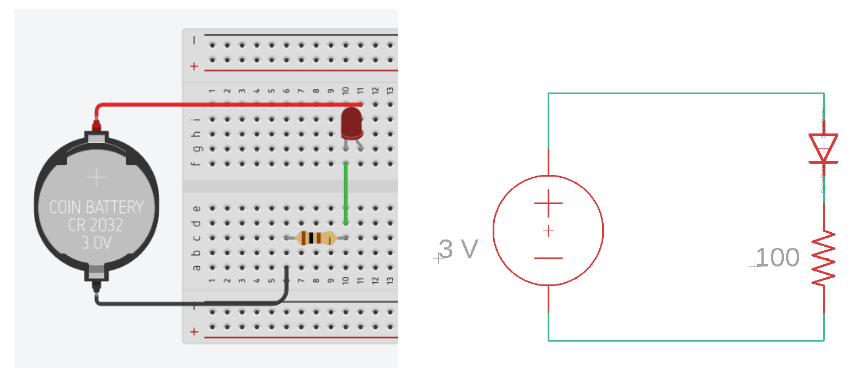
\includegraphics[width=0.85\textwidth]{./img/ckpt_1_0.png}
    \caption{Circuito b\'asico con un diodo LED y una resistencia.}
    \label{fig:circuito_basico}
\end{figure}

\begin{enumerate}
    \item \textbf{Descripción del circuito:} \\
    El circuito est\'a compuesto por una bater\'ia tipo moneda de 3V, un diodo LED conectado en serie y una resistencia de 100~$\Omega$ para limitar el paso de corriente. Luego, se conectar\'a un volt\'imetro en paralelo con el LED para medir la ca\'ida de tensión y un amper\'imetro después de la resistencia para medir la corriente que atraviesa el circuito.

    \item \textbf{¿Cu\'al es el valor de la ca\'ida de tensión en los terminales del diodo LED?} \\
    De acuerdo a la Figura \ref{fig:caida_tension}, la ca\'ida de tensión en los terminales del diodo LED es de \textbf{1.98 V}.

    \item \textbf{¿Cu\'al es el valor de corriente obtenido en el circuito?} \\
    El valor de corriente medido con el amper\'imetro fue de \textbf{9.30 mA} (miliamperios).

    \item \textbf{¿Cu\'al es la potencia consumida por el diodo LED?} \\
    Usando la fórmula $P = V \times I$, donde $V = 1.98$ V y $I = 9.3$ mA, se obtiene una potencia de aproximadamente \textbf{18.414 mW}.
\end{enumerate}

\begin{figure}[H]
    \centering
    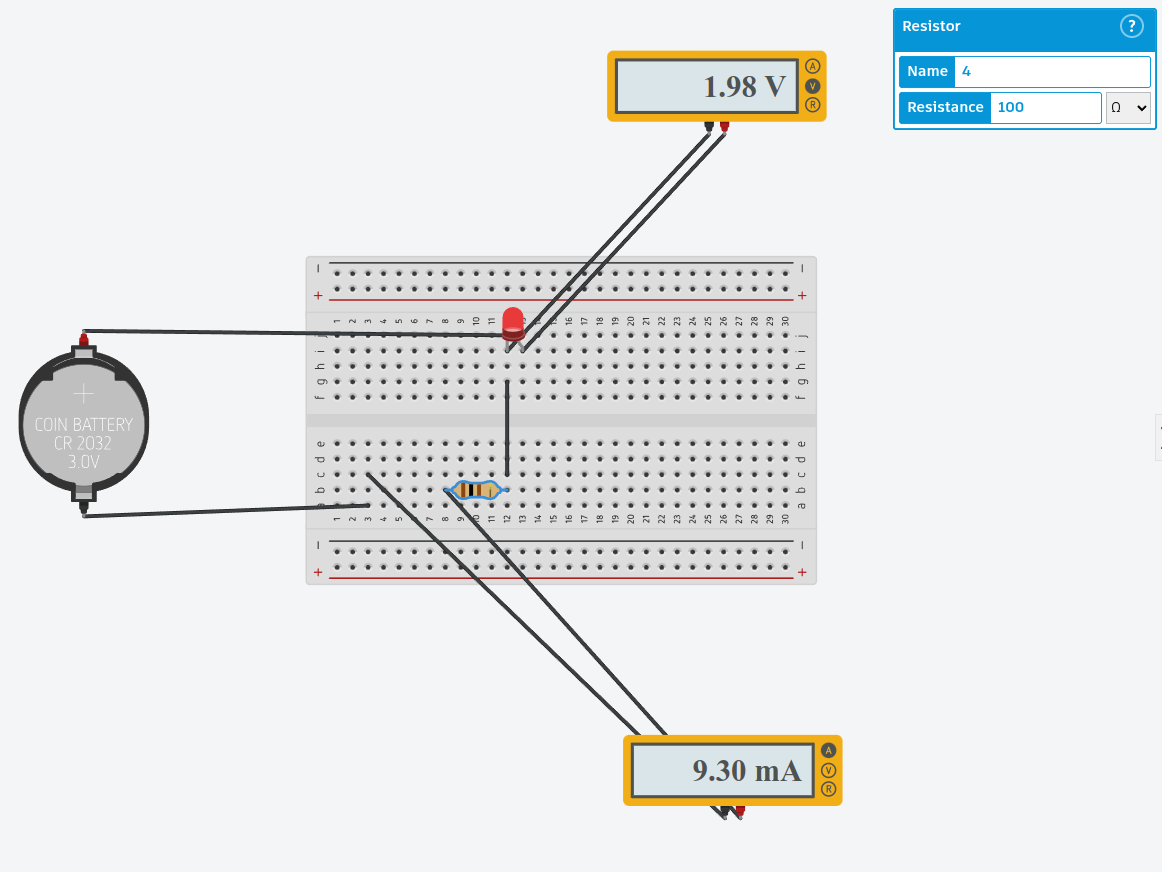
\includegraphics[width=0.85\textwidth]{./img/ckpt_1_1.png}
    \caption{Medida de ca\'ida de tensión.}
    \label{fig:caida_tension}
\end{figure}

\subsection{Checkpoint 2: Conexión de resistencias en serie y paralelo}

Similar al ejercicio anterior, se propone la implementación de 2 circuitos con resistencias en serie y paralelo.

\subsubsection{Circuito 1}

El primer circuito consiste en conectar un diodo LED simple a una resistencia como se ve en Figura \ref{fig:resistencia_serie}. Mientras que el segundo propone conectar 2 resistencias en paralelo, como se ve en la Figura \ref{fig:resistencia_paralelo}. 

\begin{figure}[H]
    \centering
    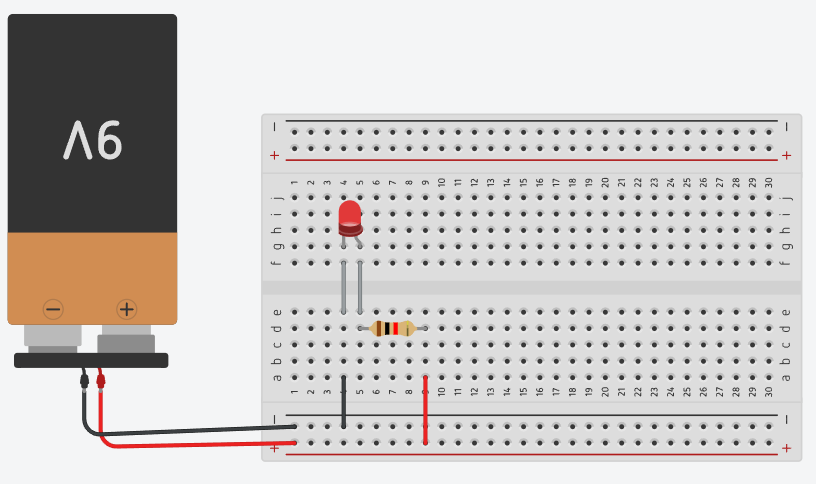
\includegraphics[width=0.5\textwidth]{./img/ckpt_2_1.png}
    \caption{Resistencia en serie}
    \label{fig:resistencia_serie}
\end{figure}


\begin{figure}[H]
    \centering
    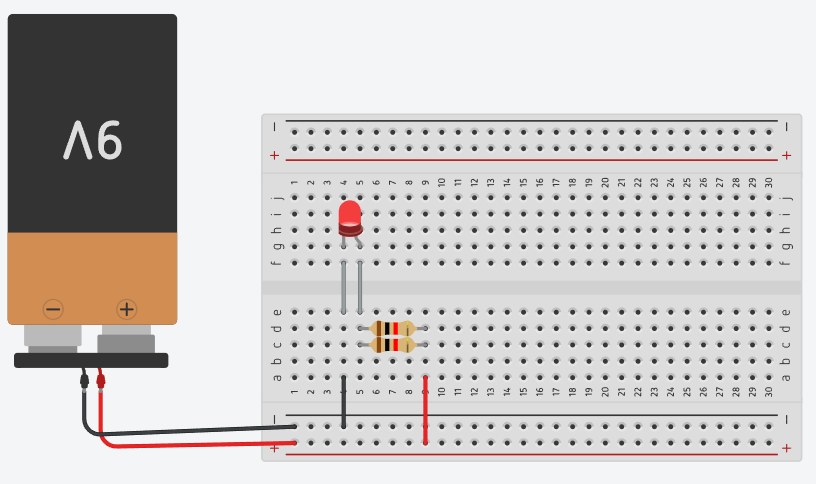
\includegraphics[width=0.5\textwidth]{./img/ckpt_2_2.png}
    \caption{2 Resistencia en paralelo}
    \label{fig:resistencia_paralelo}
\end{figure}

Ambos diodos LED se encienden, ya que las resistencias no limitan suficientemente la corriente que fluye a través de ellos. No obstante, el LED mostrado en la Figura \ref{fig:resistencia_serie} brilla con mayor intensidad en comparación con el de la Figura \ref{fig:resistencia_paralelo}, especialmente si se incrementa el valor de las resistencias.

\subsubsection{Circuito 2}

\begin{figure}[H]
    \centering
    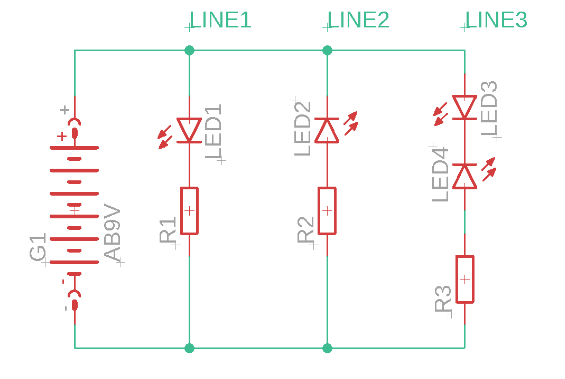
\includegraphics[width=0.5\textwidth]{./img/ckpt_2_3_0.png}
    \caption{Esquema de conexión}
    \label{fig:circuito_2}
\end{figure}

Se solicita simular (Figuras \ref{fig:simulacion_implementacion}, \ref{fig:simulacion_esquema}) en Tinkercad el esquema presentado en la Figura \ref{fig:circuito_2} y responder las siguientes preguntas:

\begin{enumerate}
    \item \textbf{Descripción del circuito:} \\
    El circuito consiste en tres ramas conectadas en paralelo a una fuente de 9V. Cada rama contiene un LED en serie con una resistencia limitadora de corriente. Esto permite que cada LED tenga su propia ca\'ida de tensión y que la corriente se divida según la resistencia y caracter\'isticas del LED en cada l\'inea.

    \item \textbf{¿Qué sucede con el diodo LED en la L\'inea 1?} \\
    El LED en la L\'inea 1 enciende correctamente. La resistencia R1 limita la corriente, permitiendo que el LED funcione dentro de su rango seguro.

    \item \textbf{¿Qué sucede con el diodo LED en la L\'inea 2?} \\
    El LED en la L\'inea 2 no enciende. Esto se debe a que la polaridad del diodo est\'a invertida, lo que impide el paso de corriente. En este caso, la resistencia R2 no limita la corriente, ya que el LED no permite que fluya.

    \item \textbf{¿Qué sucede con el diodo LED en la L\'inea 3? ¿Por qué?} \\
    Ninguno de los LEDs en la L\'inea 3 enciende. Como ambos est\'an conectados en serie, la ca\'ida de tensión total requerida (~4.4V) puede superar la tensión disponible después de la resistencia R3. Adem\'as, dado que uno de los LEDs est\'a mal conectado (polaridad invertida), este interrumpe todo el paso de corriente en esa rama, impidiendo que cualquiera de los dos encienda.
\end{enumerate}

\begin{figure}[H]
    \centering
    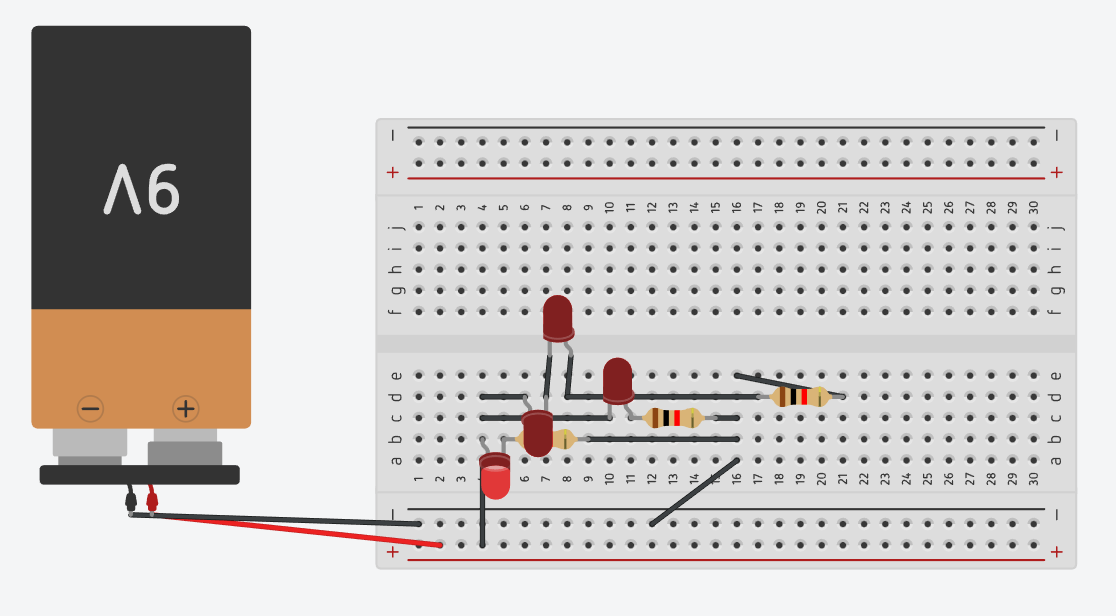
\includegraphics[width=0.85\textwidth]{./img/ckpt_2_3_1.png}
    \caption{Simulación Tinkercad del circuito.}
    \label{fig:simulacion_implementacion}
\end{figure}


\begin{figure}[H]
    \centering
    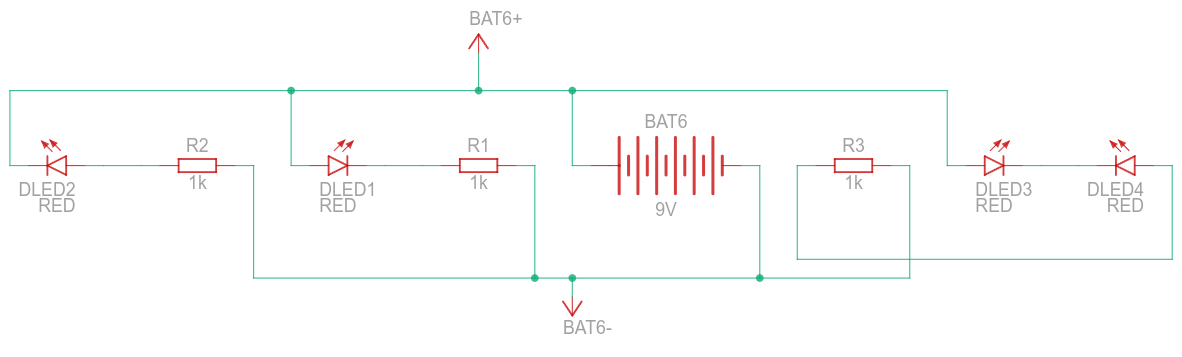
\includegraphics[width=0.85\textwidth]{./img/ckpt_2_3_2.png}
    \caption{Esquema de conexión Tinkercad}
    \label{fig:simulacion_esquema1}
\end{figure}

\subsection{Checkpoint 3: Simulación en FALSTAD}
Para el desarrollo de esta parte de la experiencia de laboratorio, nos hemos encargado de construir el siguiente circuito utilizando el programa \textbf{FALSTAD} para su simulacion.

\begin{figure}[H]
    \centering
    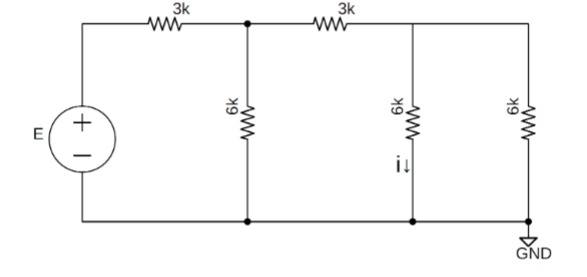
\includegraphics[width=0.85\textwidth]{./img/Circuito-3.jpeg}
    \caption{Circuito base}
    \label{fig:simulacion_esquema2}
\end{figure}

\begin{figure}[H]
    \centering
    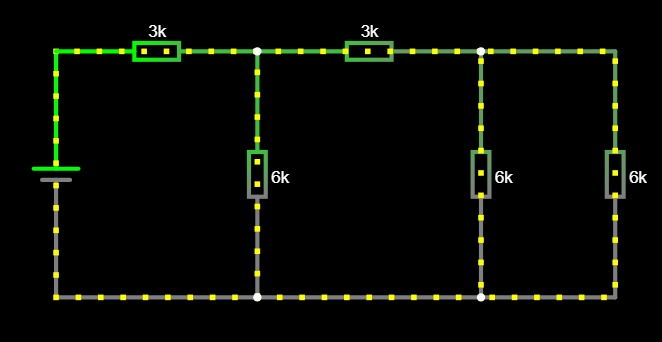
\includegraphics[width=0.85\textwidth]{./img/Falstad.jpeg}
    \caption{Circuito en simulador FALSTAD}
    \label{fig:simulacion_esquema3}
\end{figure}

Una vez realizada la simulación, hemos rescatado los siguientes datos:
\begin{itemize}
    \item El valor de la corriente ``i" es de 208.333 $\mu$A
    \item La caída de tensión en la resistencia, siendo la ultima ubicada en la derecha, de 6k tiene un valor de 1.25 V
    \item La potencia consumida por la fuente de alimentacion tiene un valor de -4.167 mW
\end{itemize}

\subsection{Checkpoint 4: LED con resistencia y potenciómetro}
En el siguiente experimento, hemos implementado el siguiente circuito, el cual nos permitira conoces mas a profundidad la funcion de un potenciometro a traves de los LEDs

\begin{figure}[H]
    \centering
    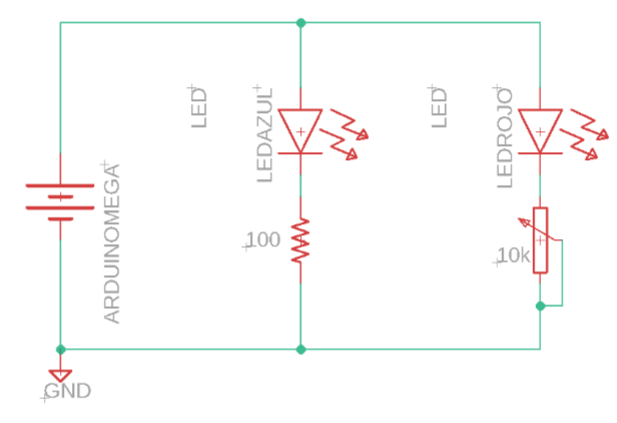
\includegraphics[width=0.50\textwidth]{./img/Circuito-potenciometro.png}
    \caption{Circuito base con potenciometro}
    \label{fig:simulacion_esquema4}
\end{figure}

A través de la implementación pudimos entender su funcionamiento y determinar lo siguiente:
\begin{itemize}
    \item El LED azul estará siempre prendido una vez inicie el flujo de corriente, debido a que este se encuentra conectado, en serie, con una resistencia de 100 ohmios, permitiendo el flujo de corriente hacia tierra.
    \item El LED rojo también se encenderá si el pin del Arduino esta en estado alto, sin embargo, su intensidad de brillo dependerá del valor ajustado en el potenciómetro de 10k ohmios
    \item Al ajustar la perilla del potenciómetro se modifica la resistencia en el circuito, lo que cambia la cantidad de corriente que fluye a través del LED. Si disminuyes la resistencia, el LED rojo brillará con mayor intensidad porque circula más corriente, en cambio, si aumentas la resistencia, el brillo del LED disminuirá hasta apagarse si se llega al minimo
    \item Si la fuente de alimentación del Arduino la cambiamos de 5 a 3.3, ambos LEDs podrían verse afectados. En primer lugar, el LED azul no se enciende debido a que estos requieren un voltaje de mínimo 3V y si sumamos la resistencia se pierde mucha corriente ocasionando esto. Por otro lado, el LED rojo si se sigue encendiendo pero con menor brillo, ya que hay menos voltaje y corriente disponibles, especialmente si el potenciómetro esta ajustado a un valor alto.
\end{itemize}

\begin{figure}[H]
    \centering
    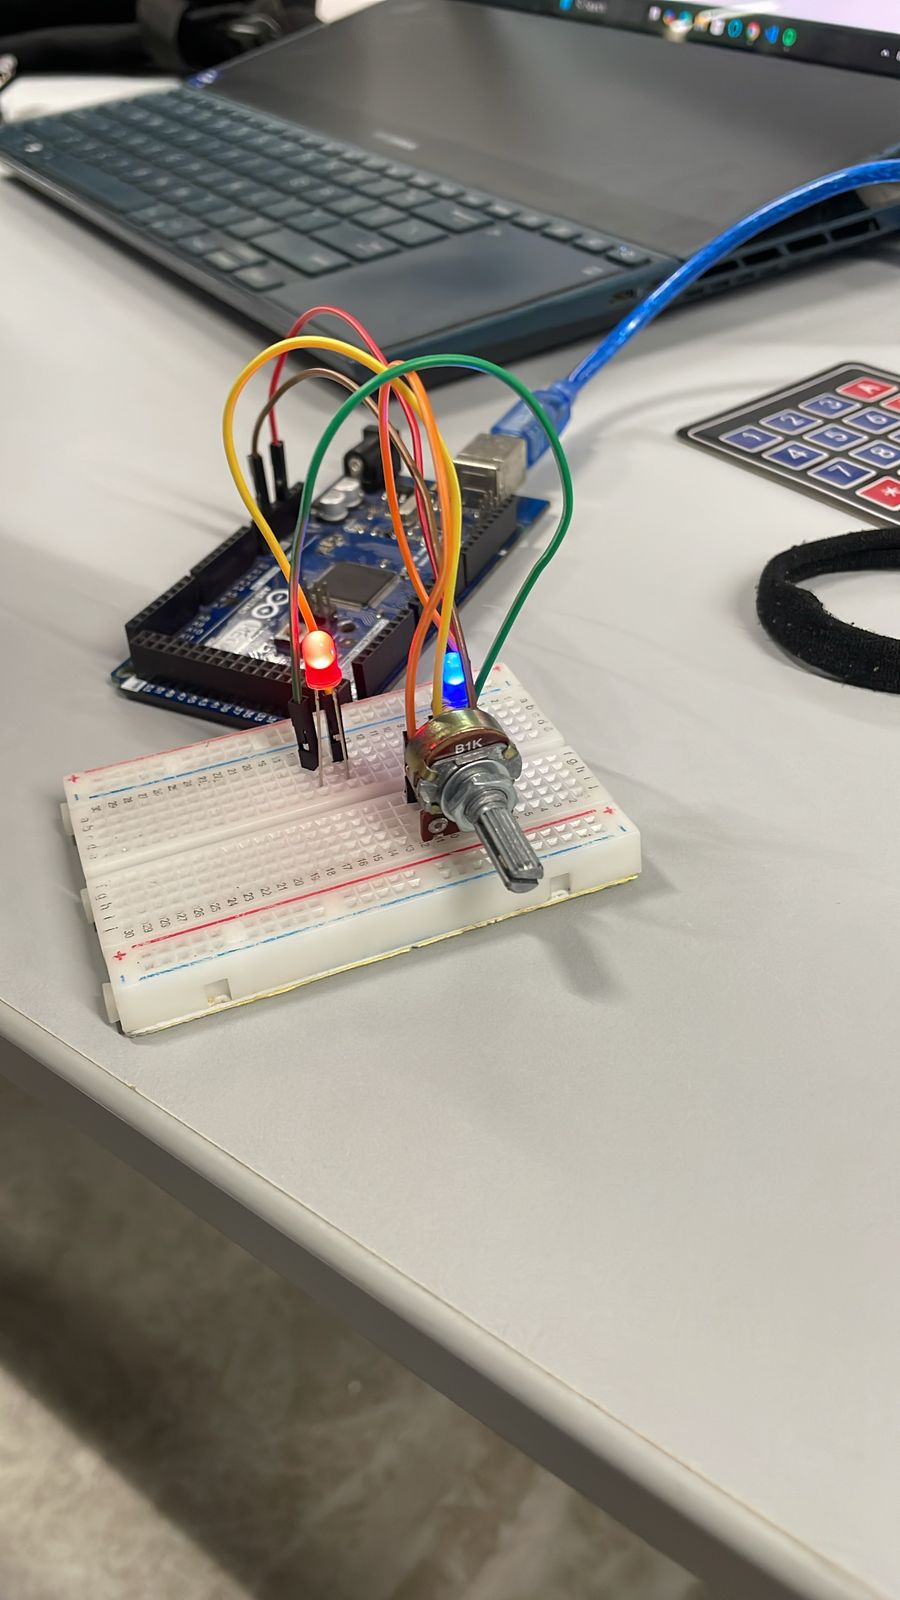
\includegraphics[width=0.50\textwidth]{./img/chkp-3-4-2.jpeg}
    \caption{Implementación LED-Potenciometro 2}
    \label{fig:simulacion_esquema5}
\end{figure}

\begin{figure}[H]
    \centering
    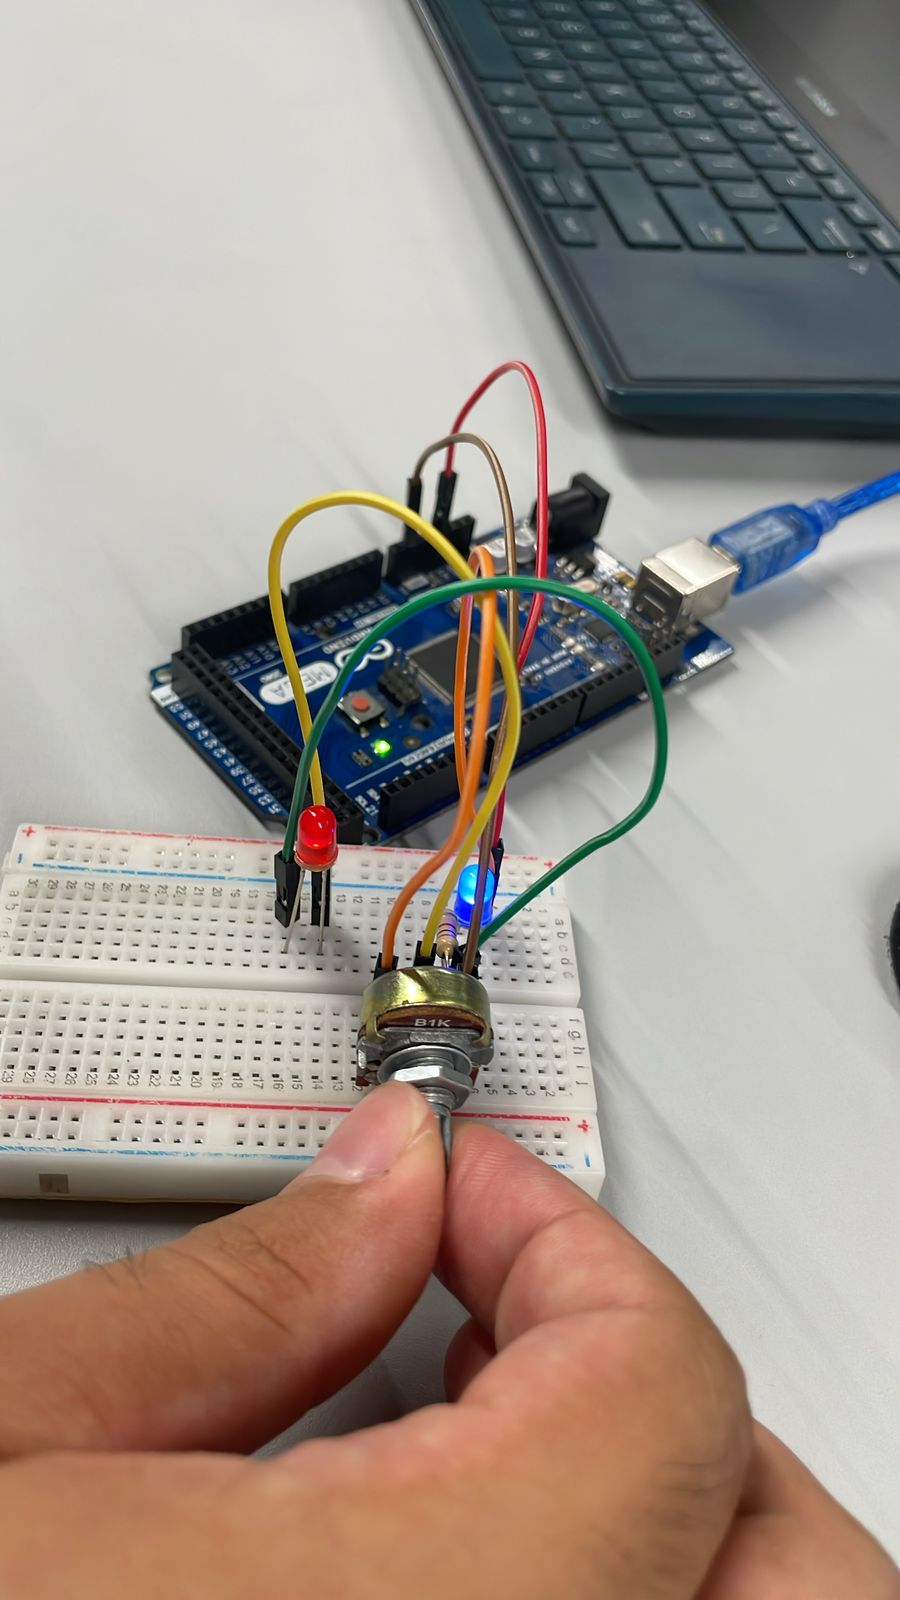
\includegraphics[width=0.50\textwidth]{./img/chkp-3-4-1.jpeg}
    \caption{Implementación LED-Potenciometro 2}
    \label{fig:simulacion_esquema6}
\end{figure}

\subsection{Checkpoint 5: Uso de un botón}
En esta sección se explora el comportamiento de un circuito digital mediante el uso de un botón configurado como entrada, empleando una conexión tipo pull-up. Esta configuración es común en sistemas embebidos, ya que permite asegurar un estado lógico definido en ausencia de interacción física. En este caso, se busca controlar el encendido de un LED utilizando un botón conectado a tierra.

\begin{figure}[H]
    \centering
    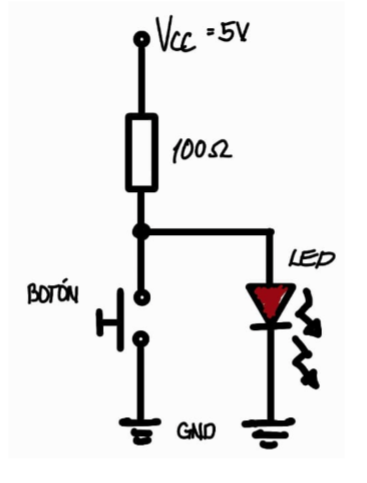
\includegraphics[width=0.50\textwidth]{./img/Circuito-boton.png}
    \caption{Circuito base con boton}
    \label{fig:simulacion_esquema7}
\end{figure}

El circuito se ha diseñado de tal manera que, por defecto, el LED permanece encendido, aprovechando que el voltaje en la salida es alto mientras el botón no es presionado. Al oprimir el botón, la salida se conecta a GND, lo que provoca que el voltaje caiga a nivel bajo y el LED se apague. Esta lógica de control resulta útil para ilustrar el funcionamiento de entradas digitales activas en bajo (active-low) y para analizar el efecto de cambiar la configuración a pull-down, lo cual invertiría completamente el comportamiento del sistema, es decir por defecto estaría apagado y al presionar el botón el circuito se cerraría cambiando a prendido.

\begin{figure}[H]
    \centering
    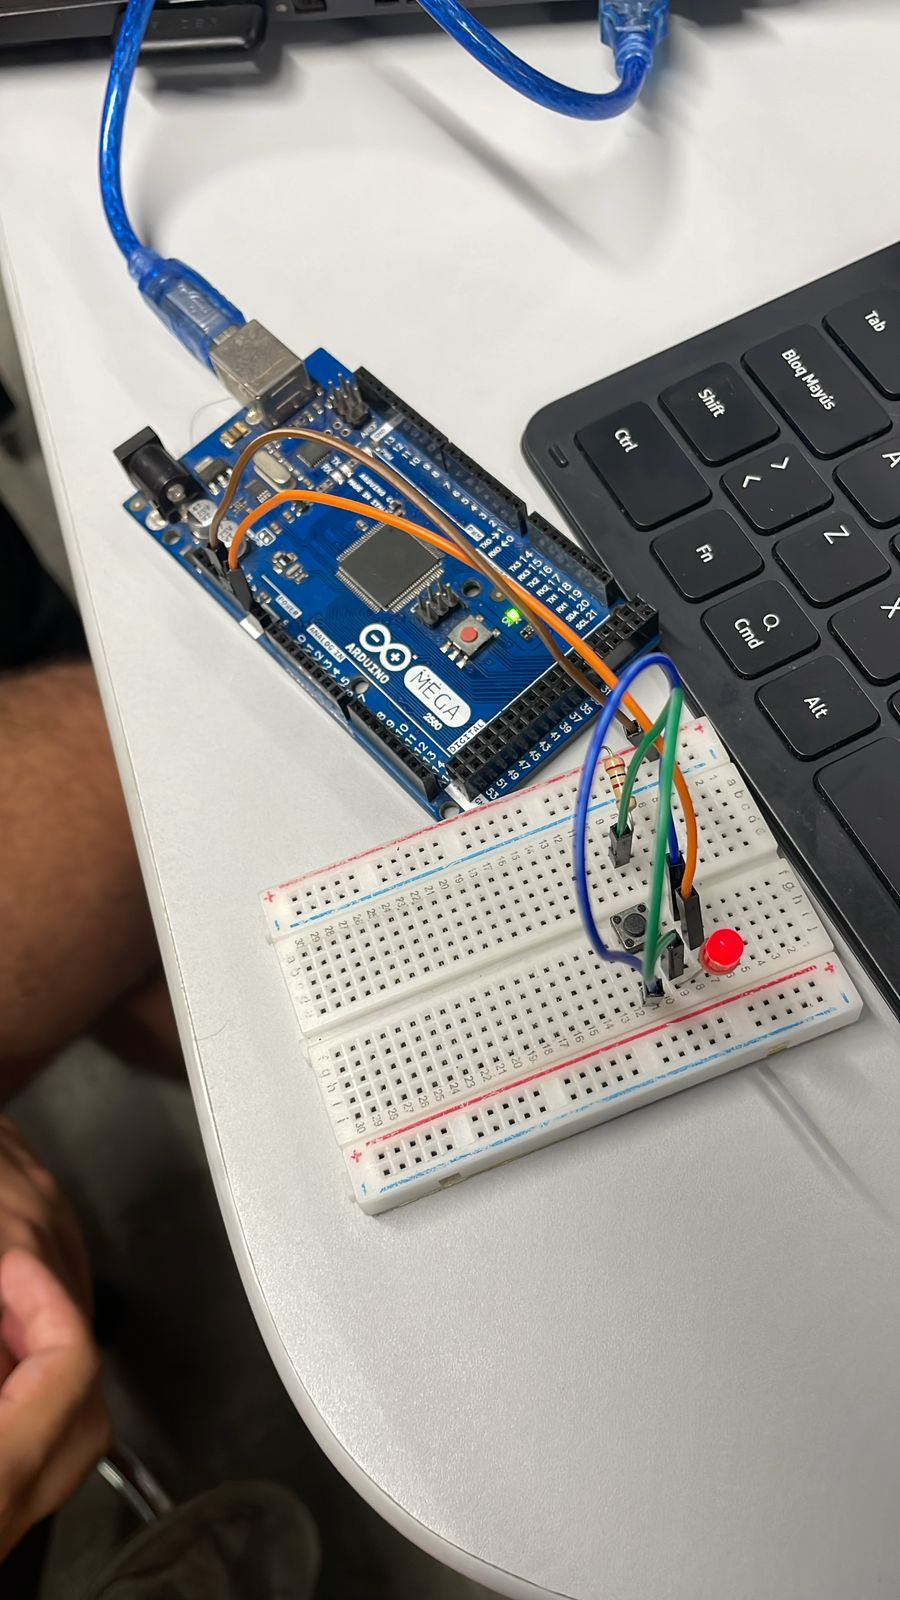
\includegraphics[width=0.50\textwidth]{./img/chkp-3-5-1.jpeg}
    \caption{Implementación del circuito con boton}
    \label{fig:simulacion_esquema8}
\end{figure}

\subsection{Checkpoint 6: LEDs secuenciales}

En este ejercicio se propone el dise\~no, simulación e implementación de un sistema que utiliza cuatro diodos LED (rojo, azul, verde y amarillo) que se encienden de manera secuencial en un orden predefinido. Adem\'as, se incluye un botón que permite cambiar la dirección de la secuencia de encendido de los LEDs de forma instant\'anea, sin necesidad de completar el ciclo actual. Este sistema busca reforzar los conceptos b\'asicos de control de hardware mediante Arduino, incluyendo el uso de salidas digitales y la lectura de entradas digitales para modificar el comportamiento del sistema.

El funcionamiento del sistema se puede dividir en dos modos: 
\begin{itemize}
    \item \textbf{Modo normal (sin presionar el botón):} los LEDs se encienden en el orden rojo → azul → verde → amarillo.
    \item \textbf{Modo inverso (botón presionado):} los LEDs se encienden en el orden amarillo → verde → azul → rojo.
\end{itemize}

La transición entre modos se realiza al detectar un cambio en el estado del botón, y la dirección del encendido cambia de inmediato, lo cual se controla mediante una variable lógica \texttt{flag}.

\begin{figure}[H]
    \centering
    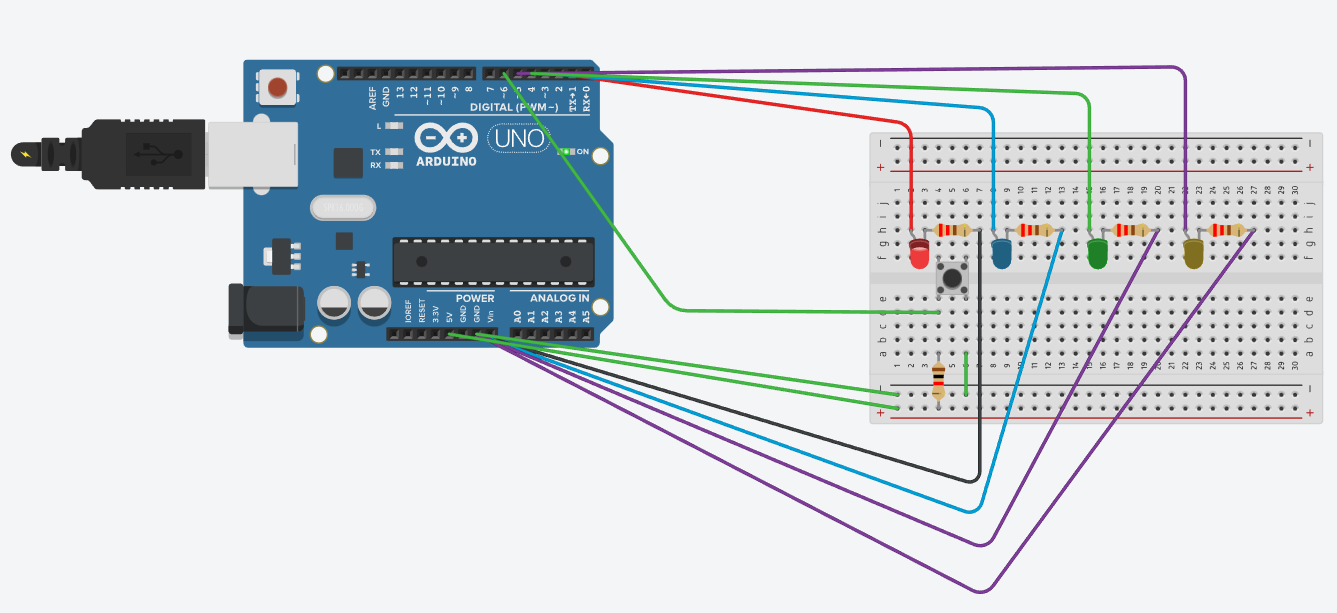
\includegraphics[width=0.85\textwidth]{./img/ckpt_6_0.png}
    \caption{Simulación Tinkercad LEDs secuenciales}
    \label{fig:leds_secuenciales}
\end{figure}

El código mostrado a continuación permite gestionar esta lógica. Cada vez que se ejecuta el bucle \texttt{loop()}, se verifica el estado del botón. Si est\'a presionado, se invierte la dirección de la secuencia. Luego, se incrementa la variable \texttt{color}, y se decide cu\'al LED encender según el valor de \texttt{color \% 4} y la dirección actual (\texttt{flag}). Al finalizar, se enciende el LED correspondiente durante un segundo y luego se apaga.


\begin{lstlisting}[style=cppstyle, caption={Código en C++ para el control de LEDs secuenciales.}, label={code:leds_secuenciales}]
// C++ code
int actual = 0, color = 0;
bool flag = 1;

void setup()
{
    pinMode(LED_BUILTIN, OUTPUT);
    pinMode(0, OUTPUT);
    pinMode(6, INPUT);
    pinMode(5, OUTPUT);
    pinMode(2, OUTPUT);
    pinMode(3, OUTPUT);
    pinMode(4, OUTPUT);
    Serial.begin(9600);
}

void loop()
{ 
    int buttonState = digitalRead(6);
    Serial.println(digitalRead(6));
    if (buttonState == LOW) flag = !flag;
    color += 1;
    if (flag)
    {
        if (color % 4 == 1) actual = 2;
        if (color % 4 == 2) actual = 3;
        if (color % 4 == 3) actual = 4;
        if (color % 4 == 0) actual = 5;
    } 
    else 
    {
        if (color % 4 == 1) actual = 5;
        if (color % 4 == 2) actual = 4;
        if (color % 4 == 3) actual = 3;
        if (color % 4 == 0) actual = 2;
    }
    digitalWrite(actual, HIGH);
    delay(1000);
    digitalWrite(actual, LOW);
}
\end{lstlisting}

Para facilitar la comprensión del algoritmo y su lógica de decisión, se elaboró el siguiente diagrama de flujo. Este representa gr\'aficamente la secuencia de decisiones y acciones que se ejecutan en el ciclo principal del programa. En él se observa cómo se lee el estado del botón, se actualiza el contador y se determina el LED que debe encenderse, de acuerdo con la dirección actual.

\begin{figure}[H]
    \centering
    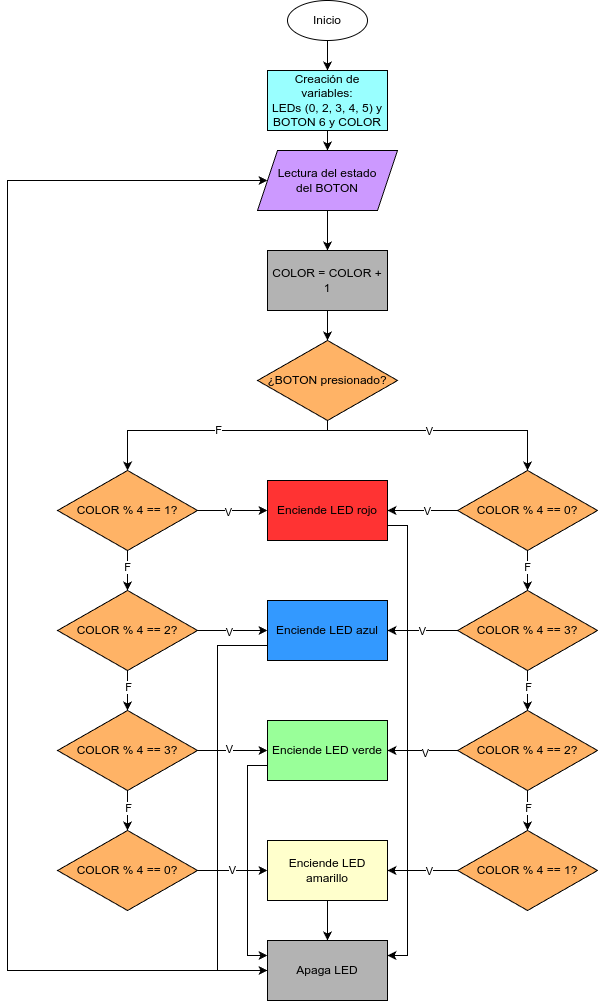
\includegraphics[width=0.6\textwidth]{./img/ckpt_6_1.png}
    \caption{Simulación Tinkercad LEDs secuenciales}
    \label{fig:leds_secuenciales_flowchart}
\end{figure}

\subsection{Checkpoint 7: Sem\'aforo}

Este ejercicio propone el diseño y la implementación de un sistema de semáforo, simulando el comportamiento real de un cruce vehicular y peatonal. El objetivo es comprender cómo gestionar múltiples salidas digitales mediante temporización, estableciendo una lógica secuencial con distintos tiempos de activación. Para ello, se controlan dos sistemas simultáneos: un semáforo de vehículos con tres estados (rojo, verde y amarillo), y un semáforo peatonal con dos estados (caminar y detenerse).

La lógica del sistema se basa en tiempos de permanencia predeterminados para cada luz (rojo: 10 segundos, verde: 5 segundos, amarillo: 2 segundos), lo que permite replicar el comportamiento típico de una intersección vial. A través del uso de estructuras de control y funciones de temporización en el entorno de Arduino, los estudiantes pueden simular y luego implementar físicamente esta lógica de control, reforzando conceptos como la sincronización de eventos, control de múltiples salidas y diseño mediante diagramas de flujo.

\begin{figure}[H]
    \centering
    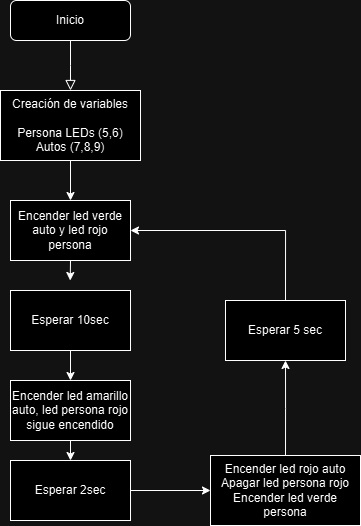
\includegraphics[width=0.6\textwidth]{./img/flujo_semaforo.png}
    \caption{Diagrama de flujo}
    \label{fig:leds_secuenciales_flowchart}
\end{figure}

\begin{figure}[H]
    \centering
    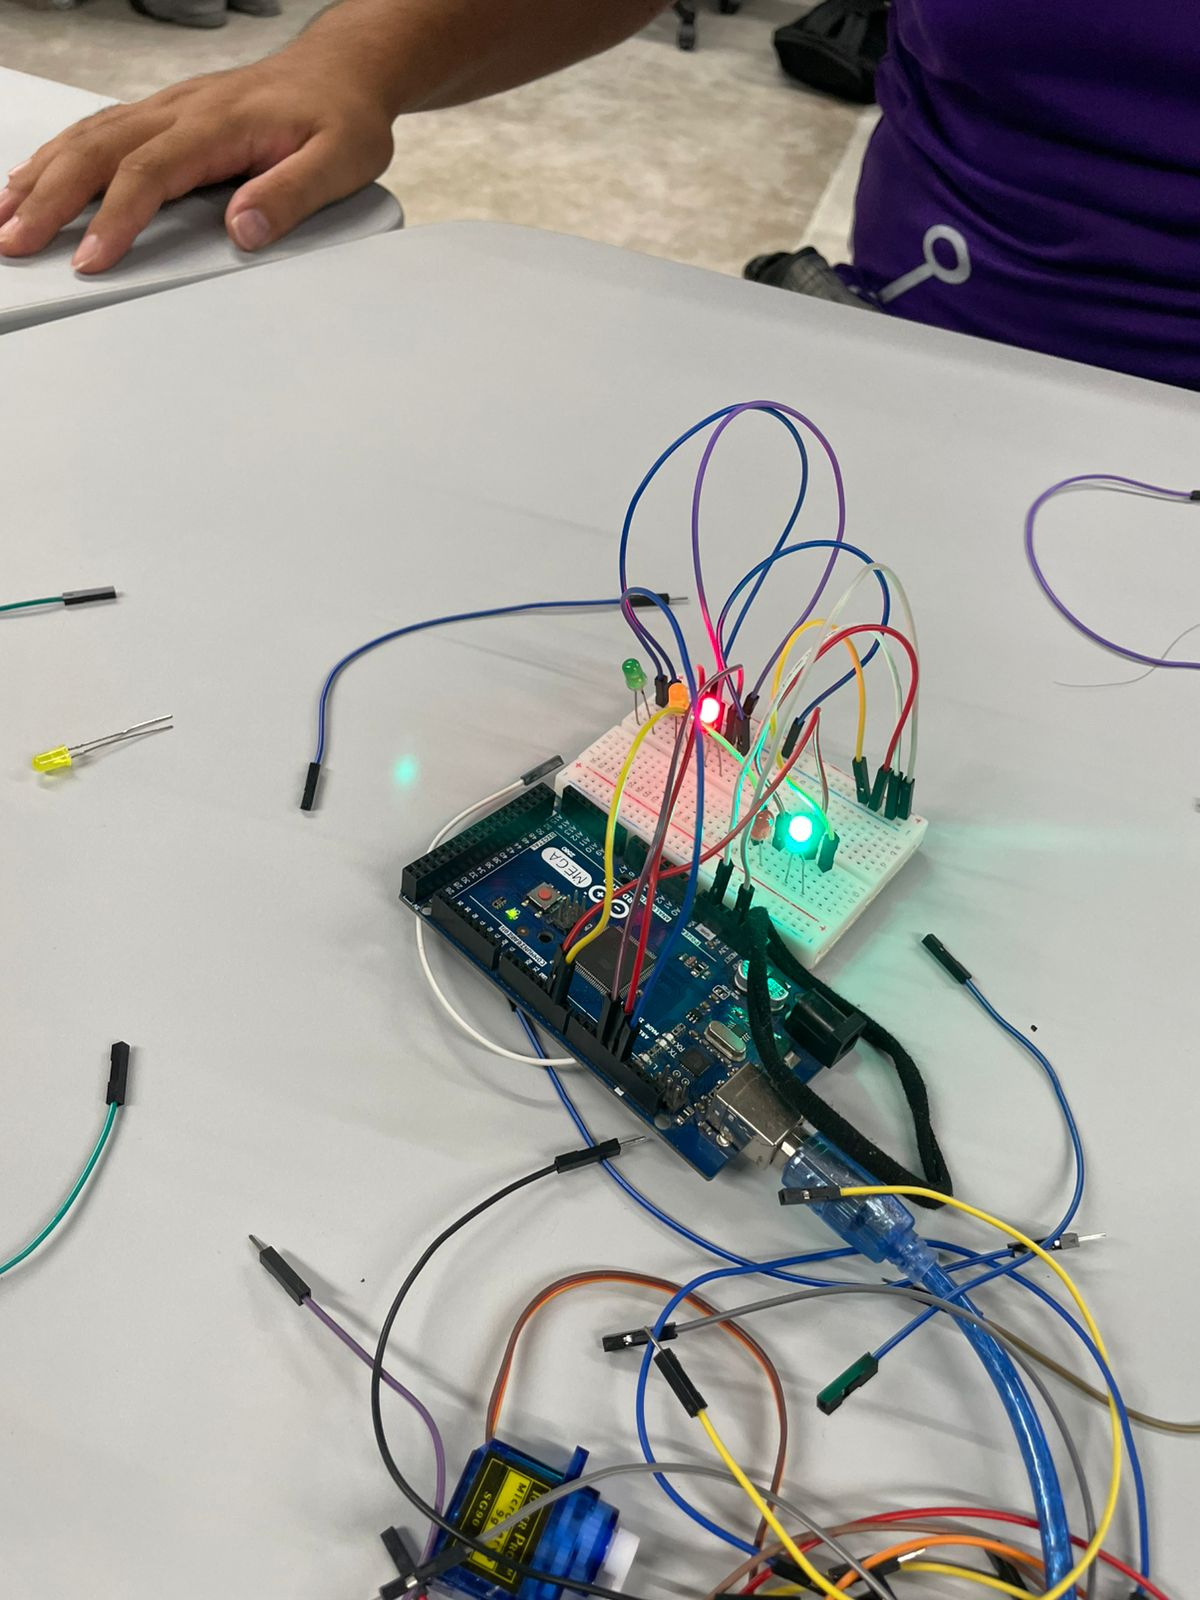
\includegraphics[width=0.6\textwidth]{./img/semaforo.jpeg}
    \caption{Implementación semáforo}
    \label{fig:leds_secuenciales_flowchart}
\end{figure}

\section{Conclusiones}

\bibliographystyle{plain}
\bibliography{bibliografia}

\end{document}

% https://tug.ctan.org/info/undergradmath/undergradmath.pdf
